\documentclass[hyperref,UTF8,12pt,a4paper]{ctexart}

\usepackage[colorlinks]{hyperref}

\usepackage{amsmath,multirow,makecell,algorithm}
\usepackage{marvosym,color}
\usepackage{ulem,wasysym}
\usepackage{forest}
\usepackage{pifont}

%Tikz画图
\usepackage{tikz}
\usetikzlibrary{arrows,graphs} %指明是图库

\usepackage{array}
\newcolumntype{P}[1]{>{\centering\arraybackslash}p{#1}}

\usepackage{geometry}
\geometry{left=1in,right=1in,top=1in,bottom=1in}

\usepackage{titling}
\pretitle{\begin{center}\fontsize{35pt}{35pt}\selectfont}
	\posttitle{\end{center}}

\forestset{
	forest-style/.style={
		for tree={
			circle,
			fill=blue!20,draw=blue!60,
			minimum size=2em,
			every node/.style={
				circle, draw,
				inner sep=0pt,
				text width=6mm,
				align=center
			}
		}
	}
}

\usepackage{enumitem}
\setenumerate[1]{itemsep=0pt,partopsep=0pt,parsep=\parskip,topsep=5pt}
\setitemize[1]{itemsep=0pt,partopsep=0pt,parsep=\parskip,topsep=5pt}
\setdescription{itemsep=0pt,partopsep=0pt,parsep=\parskip,topsep=5pt}

\usepackage{fancyhdr}

\usepackage{listings}
\usepackage{lstautogobble}  % Fix relative indenting
\usepackage{color}          % Code coloring
\usepackage{zi4}            % Nice font

\setmonofont{Consolas}

\definecolor{bluekeywords}{rgb}{0.13, 0.13, 1}
\definecolor{greencomments}{rgb}{0, 0.5, 0}
\definecolor{redstrings}{rgb}{0.9, 0, 0}
\definecolor{graynumbers}{rgb}{0.5, 0.5, 0.5}

\lstset{
    autogobble,
    columns=fullflexible,
    showspaces=false,
    showtabs=false,
    breaklines=true,
    showstringspaces=false,
    breakatwhitespace=true,
    escapeinside={(*@}{@*)},
    commentstyle=\color{greencomments},
    keywordstyle=\color{bluekeywords},
    stringstyle=\color{redstrings},
    numberstyle=\color{graynumbers},
    basicstyle=\ttfamily\footnotesize,
	frame=single,
    framesep=6pt,
    xleftmargin=30pt,
    tabsize=4,
    captionpos=b,
	language=Java,
	numbers=left,
	numbersep=15pt,
}

% 脚注
\usepackage[marginal]{footmisc}

\usepackage{algpseudocode, graphicx}

\title{SC2002 第一次讨论}
\author{pufanyi}
\date{}

\usepackage{longtable}

\begin{document}

\maketitle

\newpage

\tableofcontents

\newpage

\section{Overview}

\subsection{一些有用的链接}

\begin{itemize}
	\item \href{https://github.com/pufanyi/FYPMS}{GitHub Repository}
	\item \href{https://entuedu-my.sharepoint.com/:f:/g/personal/fpu001_e_ntu_edu_sg/Embuz9y7knpDkyns5CtpZbYB3_DFHYlSW8juG4VNlmebQw?e=0epo7C}{OneDrive}
	\item \href{https://app.diagrams.net/#G1WnqguonN8IsbEKNIC2t_wnUjkQRhu4ny}{UML Class Diagram}
	\item \href{https://junit.org/junit5/docs/current/user-guide/}{JUnit Document}
	\item \href{https://copilot.github.com/}{GitHub Copilot}
	\item \href{https://chat.openai.com/}{ChatGPT}
	\item \href{https://www.jetbrains.com/idea/}{IntelliJ IDEA}
\end{itemize}

\subsection{Techniques We Use}

\begin{itemize}
	\item GitHub
	\item JUnit 5.8.1
	\item GitHub Copilot \& ChatGPT
	\item JetBrains IntelliJ IDEA
\end{itemize}

\subsection{本次讨论目的}

\begin{itemize}
	\item 介绍一下我们的 project 的目的
	\item 介绍一下我们的 project 的大致架构
	\item 进行 \texttt{Model} 和 \texttt{Repository} 部分的分类与分工
	\item 大致理解 \texttt{Controller} 部分,完整读完题目
\end{itemize}

\subsection{Use Case Diagram}

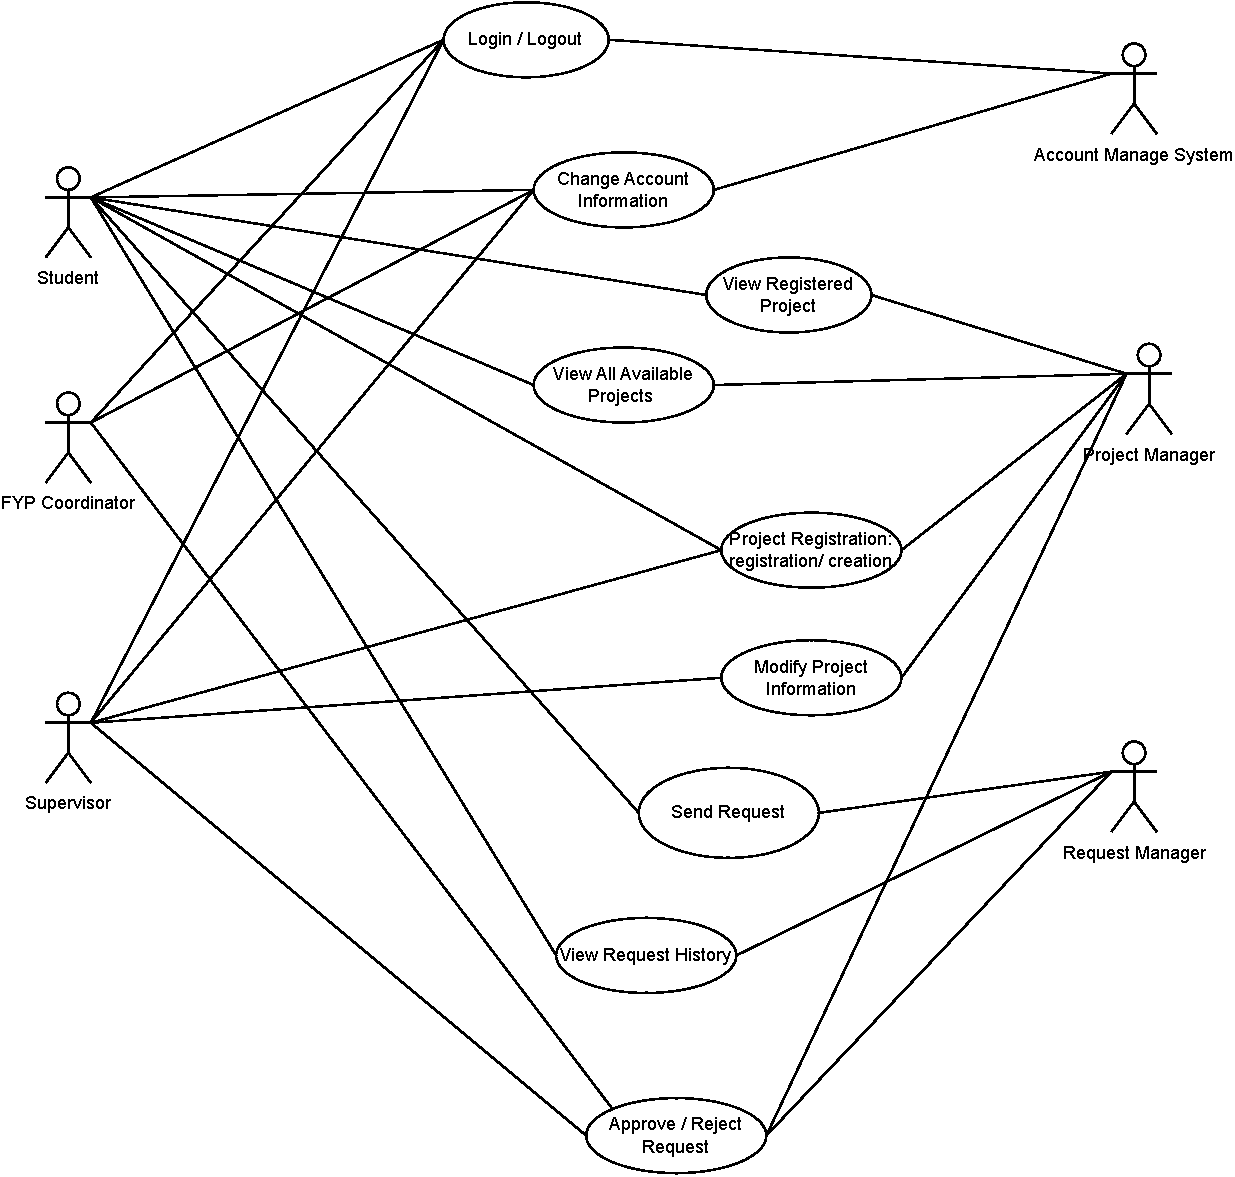
\includegraphics[width=0.8\textwidth]{diagrams/use_case_diagram.pdf}

\section{Codes}

\subsection{\texttt{Location}}

\texttt{/src/main/util/config/Location.java}

每个人都需要修改一下

代码可以复制 \texttt{/src/main/util/config/Location.java.example}

具体的,需要把其中的 \texttt{LOCATION} 改成自己整个 project 的位置。

\begin{lstlisting}[language=Java]
package main.utils.config;

public class Location {
    public static final String LOCATION = "D:\\NTU\\Y1S2\\SC2002\\FYPMS";
}
\end{lstlisting}

\subsection{\texttt{Model}}

\texttt{/src/main/model/Model.java}

具体详细的例子可以参考 \texttt{/src/main/model/user/Supervisor.java}

需要实现的 method:

\begin{itemize}
	\item \texttt{@Override public String getID()}
	\item \texttt{@Override public Map<String, String> toMap()}
	\item \texttt{@Override public void fromMap(Map<String, String> map)}
	\item \texttt{public Supervisor(Map<String, String> map)}
\end{itemize}

\subsubsection{\texttt{getID()}}

返回的是 \texttt{Model} 的 \texttt{ID},用于在 \texttt{Repository} 中进行查找。

对于同一类型的 \texttt{Model},\texttt{ID} 必须是唯一的。

\subsubsection{\texttt{toMap()}}

返回的是 \texttt{Model} 的 \texttt{Map},用于在 \texttt{Repository} 中进行存储。

\texttt{Map} 类似于 \texttt{python} 中的 \texttt{dict},可以通过 \texttt{key} 来获取 \texttt{value}。

其中我们把 \texttt{Model} 的 attribute 的 name 作为 \texttt{key},attribute 的 value 作为 \texttt{value}。

\begin{lstlisting}[language=Java]
    @Override
    public Map<String, String> toMap() {
        Map<String, String> ansMap = new HashMap<>();
        ansMap.put("supervisorID", this.supervisorID);
        ansMap.put("supervisorName", this.supervisorName);
        ansMap.put("email", this.email);
        ansMap.put("password", getPassword());
        return ansMap;
    }
\end{lstlisting}


\subsubsection{\texttt{fromMap(Map<String, String> map)}}

从 \texttt{Map} 中读取 \texttt{Model} 的 attribute。

\begin{lstlisting}[language=Java]
    @Override
    public void fromMap(Map<String, String> map) {
        this.supervisorID = map.get("supervisorID");
        this.supervisorName = map.get("supervisorName");
        this.email = map.get("email");
		setPassword(map.get("password"));
    }
\end{lstlisting}

\subsubsection{\texttt{Supervisor(Map<String, String> map)}}

通过 \texttt{Map} 来构造 \texttt{Model}。

\begin{lstlisting}[language=Java]
	public Supervisor(Map<String, String> map) {
		fromMap(map);
	}
\end{lstlisting}

\subsection{\texttt{Repository}}

具体详细的例子可以参考 \texttt{/src/main/repository/user/FacultyRepository.java}

\texttt{Repository<ModelType>} 中的 \texttt{ModelType} 是要存储的 \texttt{Model} 的类型,必须继承于 \texttt{Model} 类型。

\begin{lstlisting}[language=Java]
import main.repository.Repository;

public class FacultyRepository extends Repository<Supervisor> {
	...
}
\end{lstlisting}

需要实现的 method:

\begin{itemize}
	\item \texttt{@Override public String getFilePath()}
	\item \texttt{@Override public void seeAll(List<Map<String, String>> data)}
	\item \texttt{public FacultyRepository()}
	\item \texttt{public static FacultyRepository getInstance()}
\end{itemize}

其他方法不需要再实现,直接用即可。

\subsubsection{\texttt{getFilePath()}}

返回的是存储仓库的绝对路径。

\begin{lstlisting}[language=Java]
    final private static String FILE_PATH = "/data/user/faculty.txt";

    @Override
    public String getFilePath() {
        return Location.LOCATION + FILE_PATH;
    }
\end{lstlisting}

\subsubsection{\texttt{seeAll(List<Map<String, String>> data)}}

给你的是一个 \texttt{List<Map<String, String>>},你需要把它转换成你需要的类型。

具体的转法见 \texttt{Model.toMap(Map<String, String>)}。

\begin{lstlisting}[language=Java]
    @Override
    public void setAll(List<Map<String, String>> listOfMappableObjects) {
        for (Map<String, String> map : listOfMappableObjects) {
            getAll().add(new Supervisor(map));
        }
    }
\end{lstlisting}

\subsubsection{\texttt{FacultyRepository()}}

仿照以下方法写就好了。

\begin{lstlisting}[language=Java]
	public FacultyRepository() {
		super();
		load();
	}
\end{lstlisting}

\subsubsection{\texttt{FacultyRepository getInstance()}}

仿照以下方法写就好了。

\begin{lstlisting}[language=Java]
	public static FacultyRepository getInstance() {
		return new FacultyRepository();
	}
\end{lstlisting}

\subsubsection{\texttt{getByID}}

\begin{lstlisting}[language=Java]
    public ModelObject getByID(String modelObjectID) throws NoSuchElementException
\end{lstlisting}

\subsubsection{\texttt{contains}}

\begin{lstlisting}[language=Java]
	public boolean contains(String modelObjectID)
\end{lstlisting}

\subsubsection{\texttt{add}}

\begin{lstlisting}[language=Java]
    public void add(String modelObjectID) throws IllegalArgumentException
\end{lstlisting}

抛出 \texttt{IllegalArgumentException} 的原因是因为 \texttt{modelObject} 的 \texttt{ID} 已经存在了。

\subsubsection{\texttt{remove}}

\begin{lstlisting}[language=Java]
	public void remove(String modelObjectID) throws NoSuchElementException
\end{lstlisting}

抛出 \texttt{NoSuchElementException} 的原因是因为 \texttt{modelObject} 的 \texttt{ID} 不存在。

\subsubsection{\texttt{isEmpty}}
\begin{lstlisting}[language=Java]
    public boolean isEmpty()
\end{lstlisting}

\subsubsection{\texttt{size}}

\begin{lstlisting}[language=Java]
	public int size()
\end{lstlisting}

\subsubsection{\texttt{update}}

\begin{lstlisting}[language=Java]
	public void update(ModelObject) throws NoSuchElementException
\end{lstlisting}

将原来 \texttt{ID} 为 \texttt{modelObject} 的 \texttt{Model} 替换成 \texttt{modelObject}。

抛出 \texttt{NoSuchElementException} 的原因是因为 \texttt{modelObject} 的 \texttt{ID} 不存在。

\subsubsection{\texttt{updateAll}}

\begin{lstlisting}[language=Java]
	public void updateAll(List<ModelObject> modelObjects)
\end{lstlisting}

\subsubsection{\texttt{load}}

\begin{lstlisting}[language=Java]
	public void load()
\end{lstlisting}

从仓库中重新加载数据。

\subsubsection{\texttt{save}}

\begin{lstlisting}[language=Java]
	public void save()
\end{lstlisting}

将数据保存到仓库中。

需要注意的是,凡是已完成的方法,如果数据库中的数据发生了变化,都已经自动调用 \texttt{save()} 方法。

\subsubsection{\texttt{findByRules}}

不给出定义了,只说一下怎么用:

\begin{lstlisting}[language=Java]
    facultyRepository.findByRules(
		supervisor -> supervisor.getID().equals("A1234567A")
	);
    facultyRepository.findByRules(
		supervisor -> supervisor.getID().equals("A1234567A"),
		supervisor -> supervisor.getID().equals("12345")
	);
\end{lstlisting}

传入参数是 \texttt{modelObject -> expression} 或者 \texttt{modelObject -> \{ statements; \}},返回值是 \texttt{List<ModelObject>}。

\texttt{expression} 是一个 \texttt{boolean} 类型的表达式,\texttt{statements} 是一系列的语句,最终需要 \texttt{return} 一个 \texttt{boolean} 类型的值,类似于 \texttt{method}。

返回的东西均满足 \texttt{expression} 或者 \texttt{statements}。

如果传入多个参数,那么返回的东西均满足所有的 \texttt{expression} 或者 \texttt{statements}。

\subsubsection{遍历 Repository}

\begin{lstlisting}[language=Java]
	for (Supervisor supervisor : facultyRepository) {
		...
	}
\end{lstlisting}

\subsubsection{调用 Repository}

使用 \texttt{getInstance()} 方法来获取 \texttt{Repository} 的实例。

该实例已经被初始化和数据库同步好了,可以直接使用。

\begin{lstlisting}[language=Java]
	FacultyRepository facultyRepository = FacultyRepository.getInstance();
\end{lstlisting}

例如,在代码中要找到所有叫 \texttt{Li Yi} 的 \texttt{Supervisor},可以这样写:

\begin{lstlisting}[language=Java]
	List<Supervisor> manyLiYi = FacultyRepository.getInstance().findByRules(
		supervisor -> supervisor.getName().equals("Li Yi");
	));
	for (Supervisor supervisor : manyLiYi) {
		System.out.println(supervisor.getID());
	}
\end{lstlisting}

\subsection{JUnit}

重点:一切交给 GitHub Copilot / ChatGPT!!!

例子看 \texttt{test} 目录下的代码。

\subsection{\texttt{@NotNull}}

如果像保证一个函数的传入参数不为 \texttt{null},可以这样写:

\begin{lstlisting}[language=Java]
	public void add(@NotNull String modelObjectID) {
		...
	}
\end{lstlisting}

如果传入 \texttt{modelObjectID} 为 \texttt{null},那么会抛出 \texttt{NullPointerException}。

\end{document}

